% LaTeX layout by Jonas Kahler, jonas@derkahler.de
% HashTux SAD Document
% Group Tux:
% Aman Dirar, Jerker Ersare, Jonas Kahler, Dennis Karlberg
% Niklas le Comte, Marco Trifance, Ivo Vryashkov
% Chapter 5 - Use Case View
\chapter{Use Case View}

\begin{figure}[ht]
  \centering
  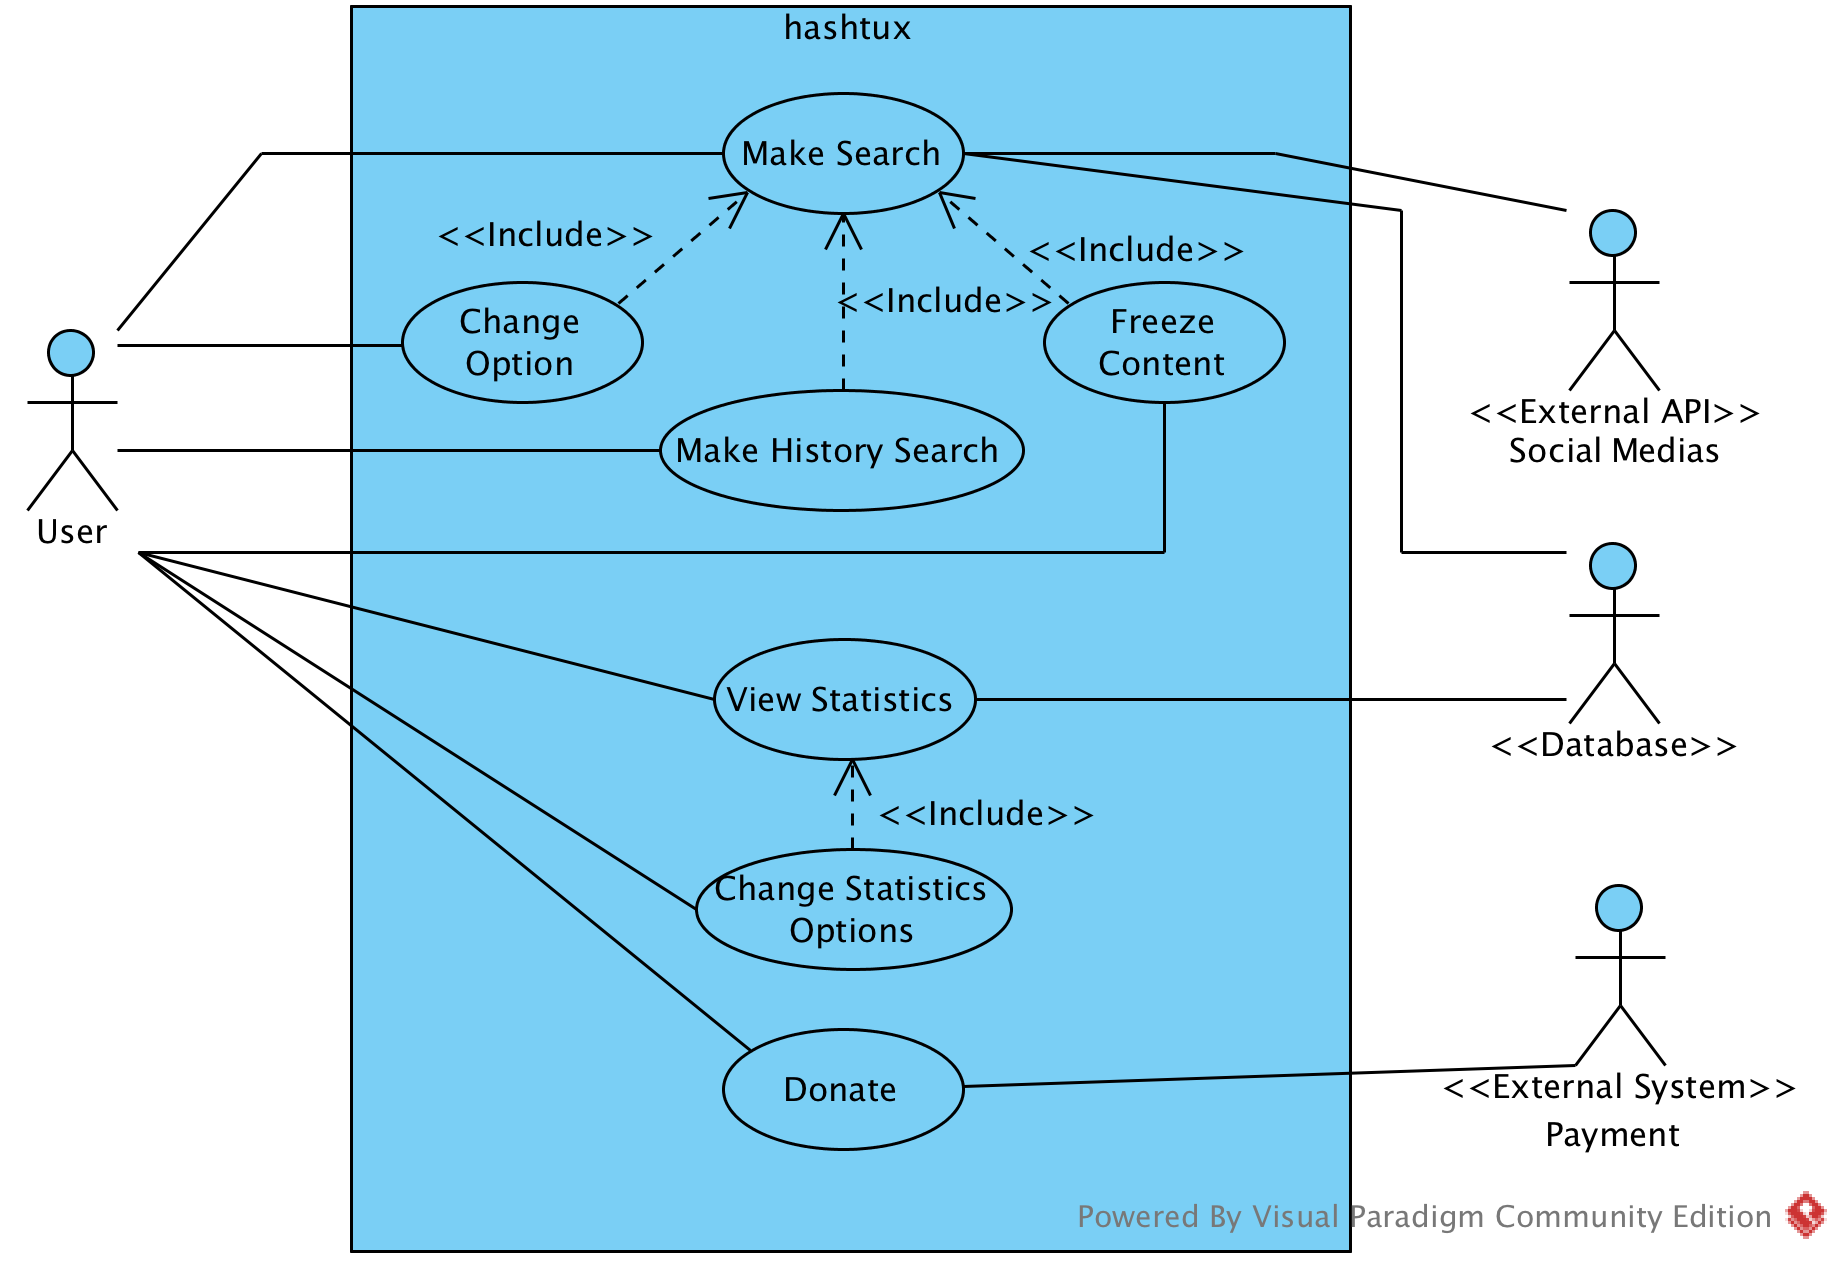
\includegraphics[width=1\textwidth]{uc_hashtux.png}
  \caption{HashTux Use Case Diagram}
\end{figure}

%% Make Search
\section{Make Search}
The user wants to search for a term to see content from the different social
media services. See the corresponding sequence diagrams in
\hyperlink{logicalview}{Logical View}.
\begin{enumerate}
  \item Basic Flow
  \begin{enumerate}
    \item The user enters a search term.
    \item The user can see the content.
  \end{enumerate}
  \item Alternative Flow
  \begin{enumerate}
    \item Starts at 1.a.
    \item There is no content for the given search term.
    \item The user enters a new search term
    \item Continues on 1.b.
  \end{enumerate}
\end{enumerate}

%%% Change Options
\section{Change Options}
The user wants to change some options for the site.
\begin{enumerate}
\item Basic Flow
  \begin{enumerate}
    \item The user selects the options menu.
    \item The user selects the preferred options.
    \item The user selects save.
    \item The user can see the new result.
  \end{enumerate}
\end{enumerate}
Precodition: \newline
Make search must have happened.

%%% Look at Past Posts
\section{Make History Search}
The user wants to look at posts from the past.
\begin{enumerate}
\item Basic Flow
  \begin{enumerate}
    \item The user selects the actions menu.
    \item The user selects the preferred timeline.
    \item The user can see the new results.
  \end{enumerate}
\end{enumerate}
Precodition: \newline
Make search must have happened.

%%% Freeze Content
\section{Freeze Content}
The user wants to freeze (pause) a post.
\begin{enumerate}
  \item Basic Flow
  \begin{enumerate}
    \item The user selects the post's freeze feature.
    \item The user can see that the post is frozen.
  \end{enumerate}
  \item Alternative Flow
  \begin{enumerate}
    \item The user selects the actions menu.
    \item The user selects the freeze feature.
    \item The user can see that the post is frozen.
  \end{enumerate}
\end{enumerate}

%%% View Statistics
\section{View Statistics}
The user wants to see user habit statistics.
\begin{enumerate}
  \item Basic Flow
  \begin{enumerate}
    \item The user enters the statistics page.
    \item The user can see the statistics.
  \end{enumerate}
  \item Alternative Flow
  \begin{enumerate}
    \item Starts after 1.a.
    \item The user selects the prefered dimension.
    \item Continues at 1.b.
  \end{enumerate}
\end{enumerate}

%%% Change Statistics Options
\section{Change Statistics Options}
The user wants to change the options for how the statistics are shown.
\begin{enumerate}
  \item Basic Flow
  \begin{enumerate}
    \item The user selects the preferred options.
    \item The user can see the results.
  \end{enumerate}
\end{enumerate}
Precondition: \newline
View Statistics must have happened.